% works on TeX-Live 2015

\documentclass{beamer}
\usepackage{tgheros}
\usepackage[varqu, scaled]{inconsolata}
%\usepackage{mylistings}
\usepackage{csquotes}
\usepackage{hyperref}
\usepackage{xcolor}
\usepackage{graphicx}
\usepackage{siunitx}
\usepackage{booktabs}
%\usepackage{tikz}
%\usepackage{tikz-uml}

% \lstset{
%   style=colored,
%   %belowskip=0pt
%   basicstyle=\ttfamily\small\color{darkgray},
%   columns=[c]fixed,
%   gobble=4
% }

% colors
\providecolor{textgreen}{RGB}{59, 158, 72}
\providecolor{textblue}{RGB}{15, 100, 255}
\providecolor{textred}{RGB}{255, 51, 66}

\usetheme[compress]{Singapore}
\useinnertheme{circles}
\setbeamercolor{structure}{fg=textblue}
%\setbeamercolor{block body alerted}{bg=normal text.bg!90!black}
\setbeamercolor{block body}{bg=normal text.bg!90!black}
%\setbeamercolor{block body example}{bg=normal text.bg!90!black}
%\setbeamercolor{block title alerted}{use={normal text,alerted text},fg=alerted text.fg!75!normal text.fg,bg=normal text.bg!75!black}
\setbeamercolor{block title}{fg=black, bg=textblue!90}
%\setbeamercolor{block title example}{use={normal text,example text},fg=example text.fg!75!normal text.fg,bg=normal text.bg!75!black}

% smaller footnotes; see: http://tex.stackexchange.com/a/192652/46356
\setbeamertemplate{footnote}{%
  \tiny%
  \parindent 1em\noindent%
  \raggedright
  \hbox to 1.8em{\hfil\insertfootnotemark}\insertfootnotetext\par%
}%
\setlength\footnotesep{0pt}

\author{Philipp Gabler}
\title{Geometry}
\date{18.\,11.\,2016}

%%%%%%%%%%%%%%%%%%%%%%%%%%%%%%%%%%%%%%%%%%%%%%%%%%%%%%%%%%%%%%%%%%%%%%%%%%%%%%%%%%%%%%%%%%%%%%%%%%%%
\begin{document}
\beamertemplatenavigationsymbolsempty

\section{Dataset}
\begin{frame}
  \begin{columns}
    \begin{column}{0.7\textwidth}
      \small
      \begin{tabular}{lrr}
        \toprule
        & Facebook\footnotemark & TX roads\footnotemark \\
        \midrule
        Vertices & 63731 & 1393383 \\
        Edges (both undir.) & 817035 & 1921660 \\
        Triangles & 3500542 & 82869 \\
        Triangles per node & 164.780 & 0.178 \\
        Mean degree & 25.640 & 2.758 \\
        Density & 0.0004023 & 0.0000002 \\
        Conn. components & 144 & 13890 \\
        Mean component size & 442.576 & 100.315 \\
        Global clustering coeff. & 0.1477 & 0.0602 \\
        \bottomrule
      \end{tabular}
    \end{column}
    \begin{column}{0.3\textwidth}
      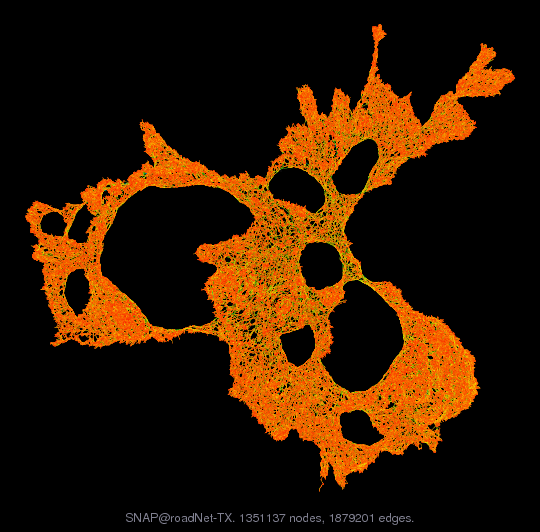
\includegraphics[width=\textwidth]{fig/texas-image}
    \end{column}
  \end{columns}
  \footnotetext[1]{\protect\url{http://konect.uni-koblenz.de/networks/facebook-wosn-links}}
  \footnotetext[2]{\protect\url{http://konect.uni-koblenz.de/networks/roadNet-TX}}

  \begin{block}{Question}
    A road network is topologically fundamentally different from a social one.  How do different
    sampling strategies react to these differences?
  \end{block}
\end{frame}


%%%%%%%%%%%%%%%%%%%%%%%%%%%%%%%%%%%%%%%%%%%%%%%%%%%%%%%%%%%%%%%%%%%%%%%%%%%%%%%%%%%%%%%%%%%%%%%%%%%%
\section{Experimental Setup}
\begin{frame}
  Comparison of \textit{random walk} and \textit{forest fire} (see
  here\footnote{\protect\href{https://cs.stanford.edu/people/jure/pubs/sampling-kdd06.pdf}{Leskovec,
      J; Faloutsos, C. \enquote{Sampling from Large Graphs.} In: Proceedings of the 12th ACM SIGKDD
      International Conference on Knowledge Discovery and Data Mining, 631--636. ACM, 2006.}}), by
  analysing some graph measures on samples.  \vspace{-0.5cm}
  \begin{columns}
    \begin{column}[t]{0.5\textwidth}
      \begin{block}{Texas}
        \centering
        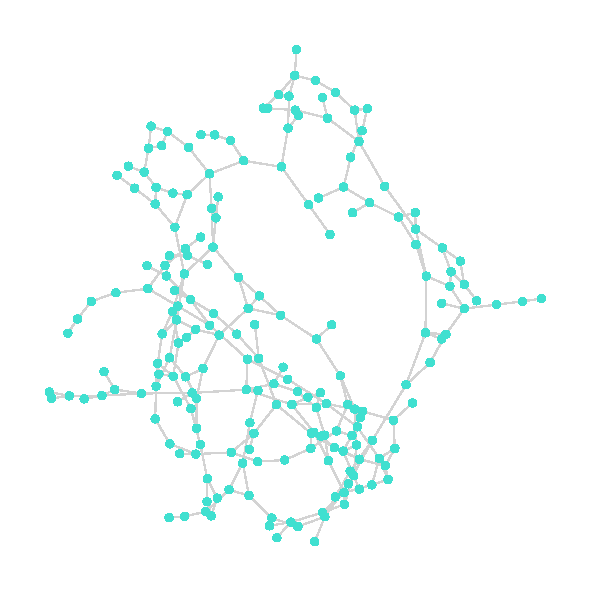
\includegraphics[scale=0.3]{fig/texas_rw}\\
        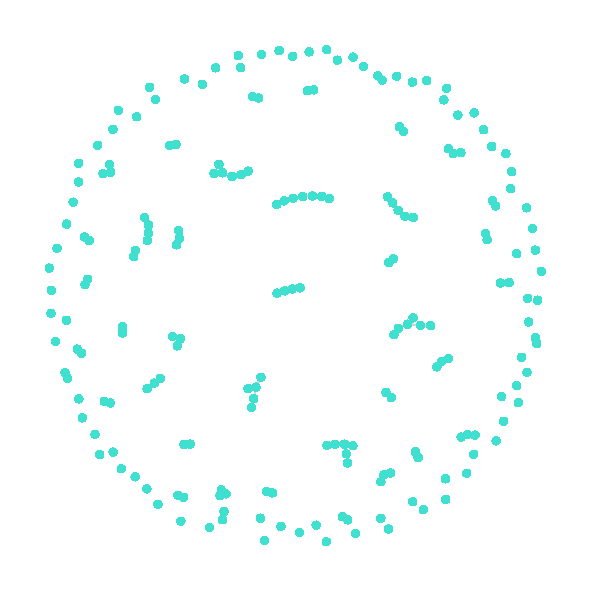
\includegraphics[scale=0.3]{fig/texas_ff}
      \end{block}
    \end{column}
    \begin{column}[t]{0.5\textwidth}
      \begin{block}{Facebook}
        \centering
        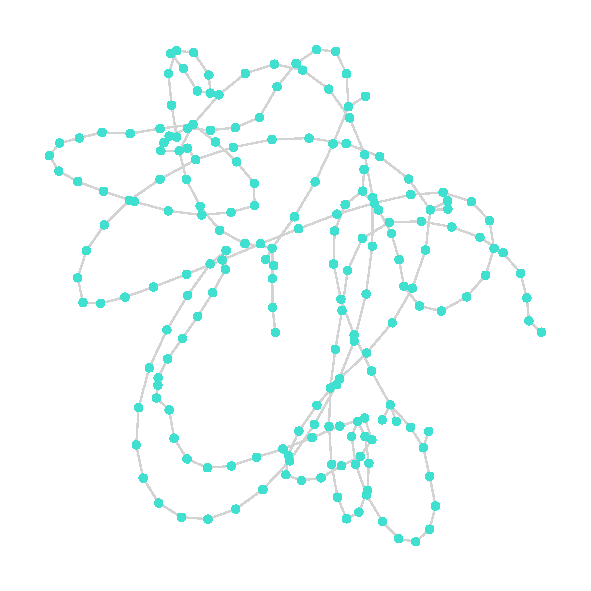
\includegraphics[scale=0.3]{fig/facebook_rw}\\
        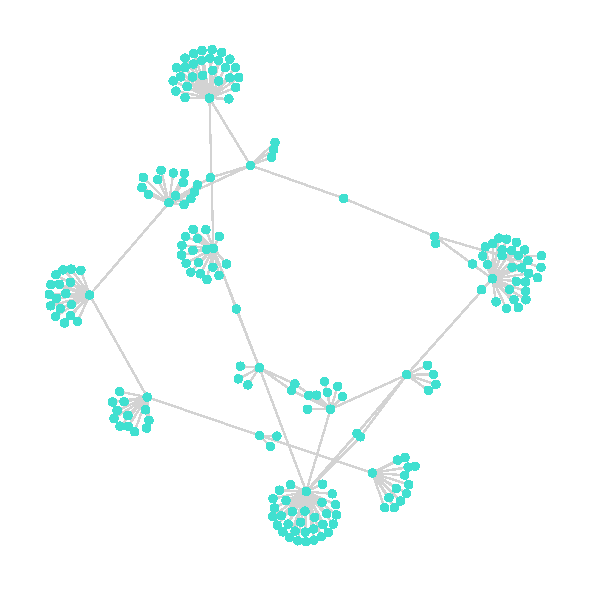
\includegraphics[scale=0.3]{fig/facebook_ff}
      \end{block}
    \end{column}
  \end{columns}
\end{frame}



%%%%%%%%%%%%%%%%%%%%%%%%%%%%%%%%%%%%%%%%%%%%%%%%%%%%%%%%%%%%%%%%%%%%%%%%%%%%%%%%%%%%%%%%%%%%%%%%%%%%
\section{Results}
\begin{frame}
  Some meaningful measures by sampling 100 times from both data sets, using 10~\% of the
  network\footnote{Code, data, and statistics:
    \protect\url{https://github.com/phipsgabler/netsci-01}}.  \vspace{1ex}
  \begin{columns}
    \begin{column}[t]{0.4\textwidth}
      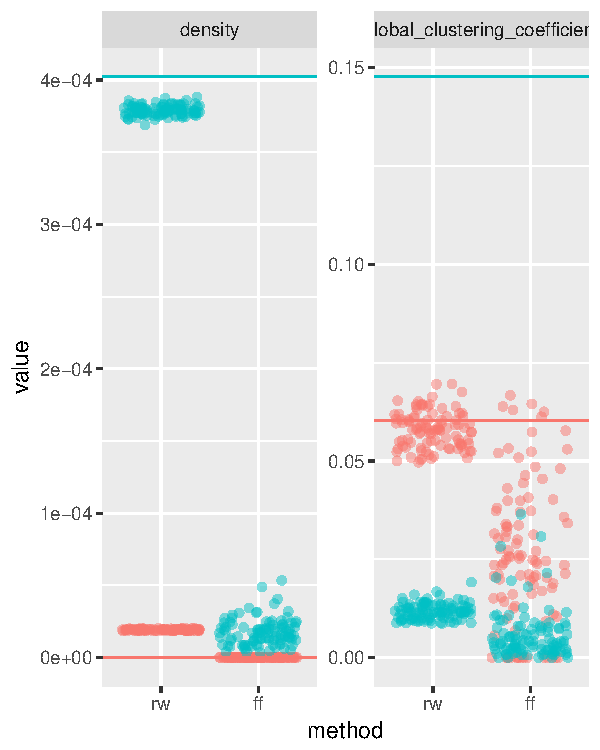
\includegraphics[width=\textwidth]{fig/sampled-ok}\\
      Magnitude mostly preserved
    \end{column}
    \begin{column}[t]{0.6\textwidth}
      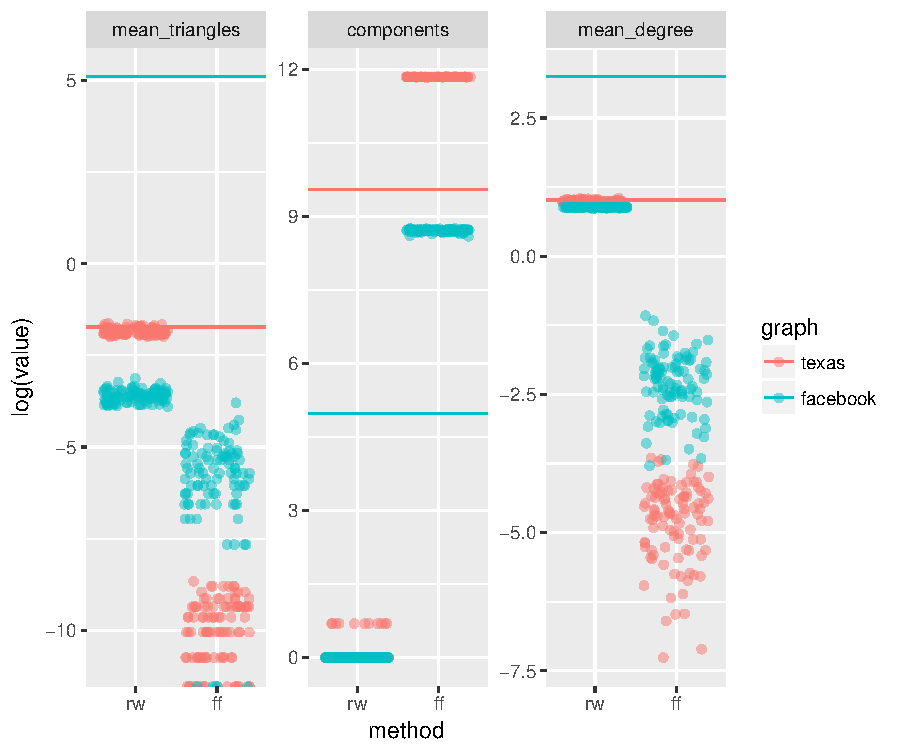
\includegraphics[width=\textwidth]{fig/sampled-off}\\
      Magnitudes far off, but order still mostly preserved
    \end{column}
  \end{columns}
\end{frame}


% @misc{snapnets,
%   author       = {Jure Leskovec and Andrej Krevl},
%   title        = {{SNAP Datasets}: {Stanford} Large Network Dataset Collection},
%   howpublished = {\url{http://snap.stanford.edu/data}},
%   month        = jun,
%   year         = 2014
% }

\end{document}